\noindent\rule{3cm}{0.2pt}

\subsection{Blueprint}
\textit{
\begin{enumerate}
    \item Describe what models will be used
    \item Briefly describe what BERT is
    \item Mention that models without BERT will be compared with the ones with BERT
    \item Performance measures
    \item Dataset selection and preparation
    \item Steps made during the modeling
\end{enumerate}
}

\noindent\rule{3cm}{0.2pt}
\\

Access to high-quality data is a significant challenge faced in data modeling and machine learning. In the absence of high-quality data, it is impossible to construct accurate machine learning models. Poor quality data, characterized by unreliable data collection methods, a large number of errors, incompleteness, or mislabeling, can compromise the effectiveness of any machine learning algorithm. This issue is particularly pertinent in the context of datasets containing fake news, where labeling is not as straightforward as with other datasets. The task of manual labeling, which is required to obtain ready-made texts labeled as fake news or real information, can be both time-consuming and challenging, requiring substantial trust in the person performing the labeling. As such, the labeling process is prone to significant human error, which can impact the selection of an appropriate dataset.

This research article aims to investigate how the use of various natural language processing (NLP) methods influences the accuracy of fake news prediction, rather than building a model to accurately predict fake news. Therefore, when selecting a dataset, the most crucial considerations are the quality of the labeled observations and the consistency of the labeled texts across the entire dataset. Additionally, the text should closely align with the research area, as the focus of this study is on detecting fake news. To construct a universal tool for detecting fake news, the dataset should include varied topics and text characteristics, reflecting the real-world distribution as accurately as possible. In this way, the model can learn from natural data, picking up the nuances present in different texts, such as writing style, formality, and topics. However, as noted earlier, the primary objective of this article is not to construct a ready-made tool but rather to examine and impact the predictive quality of different NLP methods. 

The dataset chosen to carry out the research, which meets the criteria outlined above for a good dataset, is \href{https://www.kaggle.com/datasets/clmentbisaillon/fake-and-real-news-dataset}{\textit{Fake and real news dataset}}, obtained from the Kaggle website. The dataset comprises 40,000 observations, encompassing both authentic and fake news articles. Each observation is characterized by five variables that explicate the news item, namely, the news item's title, its content, the topic it pertains to, the date of publication, and a binary label denoting if the news is fake or not. Notably, the dataset is balanced, containing an equivalent number of true and fake news items.


\begin{figure*}
\centering
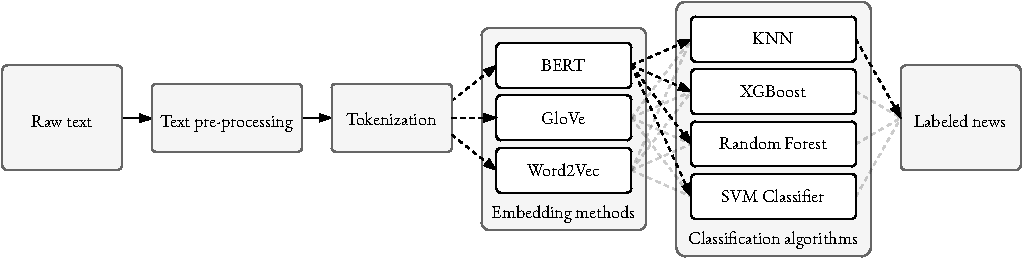
\includegraphics[width=0.8\linewidth]{methodology-schema_extended.pdf}
\caption{Architecture of each embedding-classifier model combination}
\label{methodology-schema_extended}
\end{figure*}


\subsection{Embeddings (WIP)}
\textit{Describe here what 'embedding' means and introduce embedding methods that were used in the paper...}

\subsection{Classification algorithms (WIP)}
\textit{Describe what classification algorithms has been used and what are the pros and cons for each of them...}

\subsection{Results (WIP)}

\begin{table}[hbt!]
\begin{threeparttable}
\caption{BERT Embeddings results}
\label{bert_embeddings_results}
\begin{tabular}{lll}
\toprule
\headrow Model & Accuracy & F1-Score\\
\midrule
KNN & 96.5 & 96.5\\ 
XGBoost & 95.0 & 95.0\\ 
Random Forest & 94.0 & 94.0\\ 
SVM Classifier & \textbf{98.5} & \textbf{98.5}\\ 
Logistic Regression & 98.0 & 98.0\\ 
\bottomrule
\end{tabular}
%\begin{tablenotes}[hang]
%\item[]Table note
%\item[a]First note
%\item[b]Another table note
%\end{tablenotes}
\end{threeparttable}
\end{table}

\begin{table}[hbt!]
\begin{threeparttable}
\caption{GloVe Embeddings results}
\label{glove_embeddings_results}
\begin{tabular}{lll}
\toprule
\headrow Model & Accuracy & F1-Score\\
\midrule
KNN & 89.5 & 89.4 \\ 
XGBoost & 92.5 & 92.5 \\ 
Random Forest & 87.5 & 87.4 \\ 
SVM Classifier & 94.0 & 93.9 \\ 
Logistic Regression & \textbf{94.5} & \textbf{94.4} \\ 
\bottomrule
\end{tabular}
%\begin{tablenotes}[hang]
%\item[]Table note
%\item[a]First note
%\item[b]Another table note
%\end{tablenotes}
\end{threeparttable}
\end{table}

\begin{table}[hbt!]
\begin{threeparttable}
\caption{Word2Vec Embeddings results}
\label{word2vec_embeddings_results}
\begin{tabular}{lll}
\toprule
\headrow Model & Accuracy & F1-Score\\
\midrule
KNN & 91.5 & 91.4 \\ 
XGBoost & 96.0 & 96.0 \\ 
Random Forest & 91.0 & 91.1 \\ 
SVM Classifier & \textbf{97.0} & \textbf{96.9} \\ 
Logistic Regression & 95.5 & 95.4 \\ 
\bottomrule
\end{tabular}
%\begin{tablenotes}[hang]
%\item[]Table note
%\item[a]First note
%\item[b]Another table note
%\end{tablenotes}
\end{threeparttable}
\end{table}

\begin{table}[hbt!]
\begin{threeparttable}
\caption{KNN results}
\label{knn_results}
\begin{tabular}{lll}
\toprule
\headrow Embedding Method & Accuracy & F1-Score\\
\midrule
BERT & \textbf{96.5} & \textbf{96.5} \\ 
GloVe & 89.5 & 89.4 \\ 
Word2Vec & 91.5 & 91.4 \\ 
\bottomrule
\end{tabular}
%\begin{tablenotes}[hang]
%\item[]Table note
%\item[a]First note
%\item[b]Another table note
%\end{tablenotes}
\end{threeparttable}
\end{table}

\begin{table}[hbt!]
\begin{threeparttable}
\caption{XGBoost results}
\label{xgb_results}
\begin{tabular}{lll}
\toprule
\headrow Embedding Method & Accuracy & F1-Score\\
\midrule
BERT & 95.0 & 95.0 \\ 
GloVe & 92.5 & 92.5 \\ 
Word2Vec & \textbf{96.0} & \textbf{96.0} \\ 
\bottomrule
\end{tabular}
%\begin{tablenotes}[hang]
%\item[]Table note
%\item[a]First note
%\item[b]Another table note
%\end{tablenotes}
\end{threeparttable}
\end{table}

\begin{table}[hbt!]
\begin{threeparttable}
\caption{Random Forest results}
\label{rf_results}
\begin{tabular}{lll}
\toprule
\headrow Embedding Method & Accuracy & F1-Score\\
\midrule
BERT & \textbf{94.0} & \textbf{94.0} \\ 
GloVe & 87.5 & 87.4 \\ 
Word2Vec & 91.0 & 91.1 \\ 
\bottomrule
\end{tabular}
%\begin{tablenotes}[hang]
%\item[]Table note
%\item[a]First note
%\item[b]Another table note
%\end{tablenotes}
\end{threeparttable}
\end{table}

\begin{table}[hbt!]
\begin{threeparttable}
\caption{SVM Classifier results}
\label{svc_results}
\begin{tabular}{lll}
\toprule
\headrow Embedding Method & Accuracy & F1-Score\\
\midrule
BERT & \textbf{98.5} & \textbf{98.5} \\ 
GloVe & 94.0 & 93.9 \\ 
Word2Vec & 97.0 & 96.9 \\ 
\bottomrule
\end{tabular}
%\begin{tablenotes}[hang]
%\item[]Table note
%\item[a]First note
%\item[b]Another table note
%\end{tablenotes}
\end{threeparttable}
\end{table}

\begin{table}[hbt!]
\begin{threeparttable}
\caption{Logistic Regression results}
\label{lr_results}
\begin{tabular}{lll}
\toprule
\headrow Embedding Method & Accuracy & F1-Score\\
\midrule
BERT & \textbf{98.0} & \textbf{98.0} \\ 
GloVe & 94.5 & 94.4 \\ 
Word2Vec & 95.5 & 95.4 \\ 
\bottomrule
\end{tabular}
%\begin{tablenotes}[hang]
%\item[]Table note
%\item[a]First note
%\item[b]Another table note
%\end{tablenotes}
\end{threeparttable}
\end{table}